\documentclass[a4paper,12pt]{report}
\usepackage[left=2.5cm, right=2.5cm, top=3cm, bottom=3cm]{geometry}
\usepackage[T1]{fontenc}
\usepackage{graphicx} % Required for inserting images
\usepackage{hyperref}
\usepackage{listings}
\usepackage{amsmath}
\usepackage[table]{xcolor}
\usepackage{subcaption}

\title{Linguaggi e Traduttori}
\author{Simone Petta}
\date{A.A. 2024/2025}

\lstdefinestyle{mystyle}{
    language=Python,            % Linguaggio predefinito
    backgroundcolor=\color{gray!10}, % Sfondo leggermente grigio
    basicstyle=\ttfamily\footnotesize, % Font monospace piccolo
    keywordstyle=\color{blue},   % Parole chiave in blu
    stringstyle=\color{red},     % Stringhe in rosso
    commentstyle=\color{green!50!black}, % Commenti in verde scuro
    numberstyle=\tiny\color{gray}, % Numeri di riga in grigio piccolo
    numbers=left,                % Numerazione di riga a sinistra
    stepnumber=1,                 % Numerazione per ogni riga
    showspaces=false,             % Non mostrare spazi
    showstringspaces=false,       % Non mostrare spazi nelle stringhe
    frame=single,                 % Bordo intorno al codice
    tabsize=4,                    % Dimensione del tab
    breaklines=true,              % Abilita il ritorno a capo automatico
    breakatwhitespace=true,       % Va a capo solo sugli spazi
    captionpos=b                  % Posizione della didascalia (b = bottom)
}

\lstset{style=mystyle}
\begin{document}

\maketitle
\tableofcontents

\chapter{Introduzione}
Inizio 8.45 fine 10.15

Quello che vedremo noi sono gli interpreti e in particolare riusciremo a fare un eseguibile usando un LLVM (che compila in una sorta di linguaggio macchina IR).
Esiste una libreria (che ha fatto lui) che si chiama LibLet che permette di visualizzare l'esecuzione degli algoritmi che vedremo. Tutta questa cosa sarà scritta in Python senza focalizzarci sull'orientazione ad oggetti per vedere che queste cose non si possono fare solo ad oggetti.
Vedremo anche un ripassone di algoritmi per vedere alcuni aspetti cruciali nel corso.

\section{Python}
Ci sono alcune strutture dati super comode che si possono usare con una sintassi comoda che sono le liste (strutture non omogenee), gli insiemi e i dizionari. Una cosa comoda di questi oggetti è che sono iterabili, in particolare è possibile costruire questi oggetti attraverso un meccanismo di comprehension in cui racchiudiamo tra i simboli sintattici la costruzione degli oggetti attraverso l'iterazione su un altro oggetto:

\begin{lstlisting}[language=Python]
s = [x * x for x in range(10)]
\end{lstlisting}

Se ci metto una clausola dopo questa viene valutata:
\begin{lstlisting}[language=Python]
# set comprehension: i numeri pari tra gli interi in [0, 9]
s = {x * x for x in range(9) if x % 2 == 0}
\end{lstlisting}

Si può imporre l'iterazione usando iter, notiamo che è comodo passare una sentinella per cui quando è finita l'iterazione ci ritorna la sentinella (tipicamente None):
\begin{lstlisting}
#iterazione tramite iter/next

it = iter('alcune parole divise da spazi'.split())
while True:
    w = next(it, None)
    if w is None: break
    print(w)
\end{lstlisting}

Le funzioni sono cittadini del primo ordine, possiamo assegnarle a variabili e passarle ad altre funzioni.
Le useremo per implementare in modo economico i visitor, algoritmi ricorsivi che navigano le strutture dati in modo ricorsivo per fare delle cose. In più vediamo le dispatch table (un modo comodo per fare l'object oriented) e la memorizzazione tramite i decoratori.

\begin{lstlisting}[language=Python]
def quadra(x):
    return x * x

def applica(fun, lst):
    return [fun(x) for x in lst]

applica(quadra, [1, 2, 3])
\end{lstlisting}

Noi useremo molto le liste di liste, perchè ci rappresentano gli alberi e su queste possiamo definire visite.

\begin{lstlisting}[language=Python]
lol = [1, [2, 3], [4, [5, 6]]]

#applichiamo una funzione scalare f a tutti gli elementi

def visit(f, lol):
    for elem in lol:
        if instance(elem, list):
            visit(f, elem)
        else:
            f(elem)
\end{lstlisting}

\subsection{Dispatch table}
Cominciamo a vedere un piccolo esempio di parsing di un esperessione. La prima parte del parsing è suddividere la struttura lineare del testo in chunck concettuali che non è un lavoro banalissimo:

\begin{lstlisting}
    expr = "3 + 12 * 4 + 1 * 2"
    tokens = iter(expr.split())
\end{lstlisting}

dopo di che dobbiamo definire la semantica delle operazioni, in qualche modo dobbiamo riassociare quello che osserviamo nel flusso dei token con le nostre interpretazioni. Una dispatch table è quella che associa delle informazioni a delle funzioni:

\begin{lstlisting}[language=Python]
#semantica delle operazioni, tramite la dispatch table
    def somma(x, y):
        return x + y
    def prodotto(x, y);
        return x*y
    
    DT = {
        '+': somma,
        '*': prodotto
    }
\end{lstlisting}

A questo punto se voglio valutare l'espressione usiamo in modo iterativo la dispatch table, occhio che non stiamo rispettando le regole aritmetiche, ma associamo sempre a sinistra:

\begin{lstlisting}[language=Python]
reuslt = int(next(tokens))

while True:
    t = next(tokens, None)
    if t is None: break
    of = DT[t]
    result = of(result, int(nxt(tokens)))

result
\end{lstlisting}

\subsection{Memorizzazione}
Spesso e volentieri ci capiterà di esplorare algoritmi ricorsivi per cui per risolvere un problema con un istanza grande risolveremo il problema su sue istanze più piccole, può accadere che nel processo di spezzamento andiamo a risolvere un sottoproblema che è già stato risolto da qualcun altro, quindi se non adopero accorgimenti particolari ricalcolo gli stessi risultati, l'esempio tipico è il calcolo di Fibonacci.

L'idea è salvare in una cache i risultati parziali di una funzione,

\begin{lstlisting}[language=Python]
def rendi_verbosa(f):
    def f_verbosa(x):
        result = f(x)
        print(f'f({x}) = {result}')
        return result
    return f_verbosa

def quadrato(x):
    x*x

    quadrato_verboso = rendi_verbosa(quadrato)

    q = quadrato_verboso(3)

    #tenere da parte i risultati di una funzione
    cache = {}
    
    def memoize(f):
      def f_memoized(x):
        if x not in cache: cache[x] = f(x)
        return cache[x]
      return f_memoized
\end{lstlisting}
Esiste uno zucchero sintattico con cui possiamo annotare la funzione per memorizzare i risultati parziali @memoize

\begin{lstlisting}[language=Python]
@memoize 
def cubo(x):
  return x ** 3

  cache = {}

  cubo(1), cubo(4), cubo(6)
  
  cache

  @memoize
  def fib(n):
    if n == 0 or n == 1: return 1
    return fib(n - 1) + fib(n - 2)
\end{lstlisting}

\section{Strutture dati}
Le strutture dati che vedremo sono:
\begin{itemize}
    \item alberi
    \item grafi
    \item pile/code
\end{itemize}

Gli alberi li useremo per rappresentare il testo che parseremo utilizzando una gerarchia del testo, e per visitare questa gerarchia utilizzeremo le visite.
Un altro algoritmo che useremo è il backtracking che è molto utile per comprendere gli algoritmi di parsing, è una tecnica ricorsiva che tenta di risolvere i problemi con una sorta di forza bruta ma senza infilarsi nelle chiamate ricorsive anche inutili.

\subsection{Alberi}
Gli alberi sono la struttura dati più comune del corso perchè c'è una forte ricorrenza tra linguaggi/parsing e alberi, inoltre non è difficile immaginare che molti concetti che vedremo sono rappresentabili come alberi (l'espressione aritmetica dell'altra volta).

La forma più comune che useremo è la rappresentazione con liste di liste (lol), la prima è la radice e poi ci sono i sotto-alberi con tutti i loro figli.
\begin{lstlisting}[language=Python]
# [radice] 
# [radice alberi]

tree = [1, [11, [111]], [12, [121], [122]], [13]]
\end{lstlisting}

La cosa comoda di python è che c'è l'assegnamento ordinato, viene particolare comodo l'unpacking iterabile, se metto l'* prima della variabile mi prendo tutto quello che resta:
\begin{lstlisting}
    a, *b = 1, 2, 3
    print(b) #[2, 3]
\end{lstlisting}

Questo è comodo perchè verrà comodo posso prendere i figli:
\begin{lstlisting}
    root, *children = tree
\end{lstlisting}

Come già detto useremo la libreria Liblet per visualizzare gli alberi partendo dalle lol (liste di liste).
\'E possibile fare l'unpacking anche di questi alberi con la medesima sintassi.
\begin{lstlisting}[language=Python]
from liblet import Tree, side_by_side

t = Tree.from_lol(tree)

root, *children = t
\end{lstlisting}

\subsubsection{Visite}
Quando facciamo una visita possiamo scegliere tante strategie, l'unica questione è decidere quando operare sul nodo, possiamo decidere di operare all'inizio (quando lo incontro) oppure occuparmi del nodo al termine della visita ai figli. Gli ordini vengono chiamati:
\begin{itemize}
    \item pre-ordine: visito prima il nodo e poi i figli
    \item post-ordine: visito prima i figli e poi il nodo
    \item per livello
\end{itemize}

La visita in preordine si implementa in questo modo, posto che prende la funzione che fa i suoi conti:
\begin{lstlisting}[language=Python]
def preorder(tree, root):
    root, *children = tree
    visitor(root)
    for child in children: preorder(child, visitor)
\end{lstlisting}

Per fare il postordine scambio lo scarico ricorsivo con la funzione che fa i calcoli, ovviamente visualizzeremo nodi in ordine diverso.
\begin{lstlisting}[language=Python]
def postorder(tree, visitor):
    root, *children = tree
    for child in children: preorder(child, visitor)
    visitor(root)
\end{lstlisting}

Nel caso degli alberi è possibile visitarli anche per livelli, si chiama level order. \'E un algoritmo che non fa uso della ricorsione, generalmente si adopera una coda in cui accumulo i figli che vedo in modo tale che mi occupo per primo di quelli che metto dentro:

\begin{lstlisting}
    def levelorder(tree, visitor):
        Q = queue()

        Q.enqueue(tree)
        while Q:
            tree = Q.dequeue()
            root, *children = tree
            visitor(root)
            for st in children: Q.enqueue(child)
\end{lstlisting}

\subsubsection{Alberi con attributi}

Una cosa che potrebbe essere molto comoda è che potremmo avere bisogno di usare nodi con informazioni più strututrate per poter visualizare alberi arricchiti di attributi. Per fare questo useremo un albero che abbia dict come valori e che conservi il valore numerico come valore della chiave val:
\begin{lstlisting}[language=Python]
 def add_attr(tree):
  root, *children = tree
  return [{'val': root}] + [add_attr(child) for child in children]

tree = [1, [11, [111]], [1200, [121], [122]], [13]]

add_attr(tree)
\end{lstlisting} 

Gli attributi generalmente vengono calcolati, ad esempio la profondità a cui siamo. Il modo in cui si calcolano segue due direzioni:
\begin{itemize}
    \item Attributi ereditati: calcolati per il papà e ereditati dai figli. Si usa una visita in pre-ordine.
    \item Attributi sintetizzati: in qualche modo otteniamo prima le informazioni sui figli e poi sintetizziamo verso l'alto (tipicamente la valutazione delle espressioni è un attributo sintetizzato). Si usa una visita in post-ordine, perchè prima devo visitare i figli.
\end{itemize}

Ad esempio vediamo come spingere in giù la profondità del nodo, (nella visita ricevo che sono figlio di un nodo profondo 4), quello che fa il visitor è aggiornare quella profondità di 1 per vedere quanto è profondo lui:
\begin{lstlisting}
def preorder_with_value(tree, visitor, value = None):
  root, *children = tree
  visitor(root, value)
  for child in children: preorder_with_value(child, visitor, root['depth'])

# visitor che aggiunge l'attributo depth (pari a 1 + il valore ereditato, il caso None riguarda la radice)

def add_depth(root, value):
  root['depth'] = value + 1 if value is not None else 0

attr_tree = add_attr(tree)

# la radice ricevera None perche e' il valore di default di value

preorder_with_value(attr_tree, add_depth) 

Tree.from_lol(attr_tree)
\end{lstlisting}

Nella sintesi il codice è più semplice da scrivere perchè possiamo usare il return per ritornare il valore al padre:
\begin{lstlisting}
 def postorder_with_return(tree, visitor):
  root, *children = tree
  values = [postorder_with_return(child, visitor) for child in children] # sara' la lista vuota se non ci sono figli
  return visitor(root, values)

# visitor che aggiunge l'attributo max (pari al massimo tra il valore del nodo e quelli sintetizzati dai figli)

def add_max(root, values):
  root['max'] = max([root['val']] + values)
  return root['max']

attr_tree = add_attr(tree)

postorder_with_return(attr_tree, add_max)

Tree.from_lol(attr_tree)
\end{lstlisting}

\subsection{Grafi}
Li avremo i grafi come strumenti, meno concretamente ma avremo delle visite per passare da uno stato all'altro ma non scriveremo esplicitamente grafi.
Esistono grafi non orientati e orientati. Idealmente noi useremo i grafi orientati. Tipicamente i grafi si rappresentano con:
\begin{itemize}
    \item Matrice di adiacenza, NxN dove metto true e false dove c'è un collegamento. \'E O(1) per il costo computazionale ma $O(n^2)$ nello spazio.
    \item Tengo tutte le coppie di nodi collegati se la matrice è sparsa (lista dei nodi)
    \item Tengo le liste di adiacenza di ogni nodo, per ogni nodo tengo in una lista tutti i nodi che ha collegati
\end{itemize}

Le rappresentazioni più comode che usiamo sono la rappresentazione con lista di archi (una tupla di tuple) oppure le liste di adiacenza rappresentata da un dict di set:
\begin{lstlisting}
# dagli archi alla mappa delle adiacenze


# per ogni nodo n (sia s o t), adjacency[n] = set()

adjacency = dict()
for s, t in arcs:
  adjacency[s] = set()
  adjacency[t] = set()

# aggiungo gli outlink

for s, t in arcs: adjacency[s] |= {t}

adjacency
\end{lstlisting}

\subsubsection{Algoritmi}
La visita di un grafo è un procedimento che ci porta da un nodo ad esplorare tutti gli altri, ho in qualche modo bisogno di salvarmi da qualche parte i nodi che ho visitato e quelli che devo visitare. Immaginiamo di avere bisogno di una sacca in cui mettere le cose che abbiamo bisogno di fare (ci mettiamo dentro i figli dei nodi), dobbiamo stare attenti a non rimettere dentro quello che ci è già entrato e ha senso tirare fuori gli elementi in un certo ordine:
\begin{itemize}
    \item FIFO: il primo nodo che metto è il primo che tolgo, i nodi sono messi in una coda. \'E la storia del level ordre. Così effettuiamo una visita in ampiezza.
    \item LIFO: last in first out, è una pila. Effettuiamo così una visita in profondità.
\end{itemize}

Nella visita in profondità si può dare una implementazione ricorsiva (perchè la pila può essere la pila delle chiamate), quello che dobbiamo avere è una struttura dati che ci tiene quello che abbiamo già visto, per evitare di visitare di nuovo gli stessi nodi:
\begin{lstlisting}
 def depthfirst(adjacency, start, visit):
  def walk(src):
    visit(src)
    seen.add(src)
    for dst in adjacency[src]:
      if dst not in seen: 
        walk(dst)
  seen = set()
  walk(start)
\end{lstlisting}

La visita in ampiezza usa la coda, toglo dalla coda e lo visito e quando lo vistio lo aggiungo:
\begin{lstlisting}
from liblet import Queue

def breadthfirst(adjacency, start, visit):

  Q = Queue()

  seen = set()
  Q.enqueue(start)
  while Q:
    src = Q.dequeue()
    visit(src)
    seen.add(src)
    for dst in adjacency[src]:
      if dst not in seen:
        Q.enqueue(dst)
\end{lstlisting}

Quello da notare nelle visite è che quello che succede nelle visite in profondità è che la pila non aumenta tanto di dimensione, l'unico problema è che se devo vedere nodi vicini è possibile che per visitarlo potrei dover fare un sacco di conti prima di arrivare a visitare quello. 
La visita in ampiezza d'altro canto è vero che procede per livelli, ma se il grafo è denso la coda può diventare molto grande. Quindi quello che dovremo vedere negli algoritmi di parsing è questa scelta, scendo velocemente nel grafo sperando nel successo oppure è meglio scendere per passi? quello che vedremo è che in generale se non ci sono grandi strategie l'ampiezza è l'unica strada mentre se ho qualcuno che mi dice qualcosa è meglio andare giù veloce nella strada giusta.

\subsection{backtracking}
L'idea è che possiamo decidere che alcuni rami dell'albero sono buoni e altri sono cattivi. Quindi l'idea è che se mi trovo in una strada in cui posso prevedere che se sono in un certo punto in cui non c'è speranza che andando avanti nella ricorsione non troverò mai il risultato allora posso tagliare quel ramo dell'albero. Ho una specie di soluzione parziale che posso piazzare.

Ho una soluzione candidata e se sono già capace di sapere se quella soluzione non va bene allora ritorno, se ho trovato il risultato lo stampo. Altrimenti vado avanti e faccio le chiamate ricorsive.

\begin{lstlisting}
def backtrack(candidate):
    if reject(candidate): return
    if accept(candidate): output(candidate)
    s = first(candidate)
    while s:
        backtrack(s)
        s = next(candidate)
\end{lstlisting}

Come esempio vediamo come si segmentano le parole, che è un problema fondamentale nei motori di ricerca. Inanzitutto mi procuro un elenco di parole, se segmenti non è vuota e l'ultima parola del dizionario non è in WORDS butto via, altrimenti se non mi rimane niente ho trovato tutti, altrimenti provo a spaccare in due la seguente parole in tutti i modi possibili:
\begin{lstlisting}
from urllib.request import urlopen

# WORDS sono le parole di almeno 2 caratteri (3 conta anche l'a-capo)

with urlopen('https://raw.githubusercontent.com/napolux/paroleitaliane/master/paroleitaliane/60000_parole_italiane.txt') as url: 
  WORDS = {word.decode().strip().upper() for word in url if len(word) >= 3}

print(len(WORDS))

def segmenta(segmenti, resto):
  if segmenti and not segmenti[-1] in WORDS: return
  if not resto: 
    print(segmenti)
    return
  for i in range(1, 1 + len(resto)):
    segmenta(segmenti + [resto[:i]], resto[i:])

segmenta([], 'ILCORRIEREDELLASERAEDIZIONENOTTURNA')
\end{lstlisting}


\chapter{Linguaggi}
\section{Closed form}

L'idea di poter definire un sotto-linguaggio per ciauscun simbolo è molto comodo perchè posso partire da un linguaggio e usare quello.
Il linguaggio prodotto è il prodotto dei linguaggi, la production independent è una cosa che utilizziamo molto.
Le context-free consentono una struttura che viceversa perdiamo se andiamo nel linguaggi regolari ed è la questione del self embedding.

\subsection{Self embedding}
Si intende come regola ricorsiva quando nel lato destro della produzione compare il simbolo non terminale che si sta definendo:
\begin{align*}
    A &\to aAa
\end{align*}

La regola ricorsiva è l'ingrediente necessario per rendere i nostri linguaggi infiniti.
Questa regola ci serve ad esempio ad avere il linguaggio di Dyck, che è un linguaggio di parentesi ben formate.
\begin{align*}
    A &\to ( A ) 
\end{align*}
E questo ci porta a definire correttamente un linguaggio di programmazione.
Il Context-Free è un ragionevole punto di incontro tra un linguaggio regolare e un linguaggio ricorsivo (basso ed alto livello).

\section{Alberi di parsing}
L'albero cattura la forma gerarchica di un linguaggio, è un modo per rappresentare la struttura di un linguaggio. Sia a fini linguistici sia per rappresentare la struttura di un linguaggio di programmazione.

Prima di poterci dedicare in maniera serena a questi alberi di parsing dobbiamo fare un po' di pulizia perchè abbiamo delle grammatiche con difetti che vorremmo eliminare. La spazzatura che può rimanere dentro una gramamtica context free è che possiamo avere dei non terminali non definiti. Cioè abbiamo messo dentro delle variabili (lettere maiuscole) che non abbiamo definito, non stanno mai a sinistra di una produzione. Questo è un problema perchè non possiamo mai terminare la produzione. Sono inutili e vanno eliminati. Ci sono altre due circostanze in cui ci sono problemi, potremmo avere definito un terminale che non è mai raggiungibile da nessuna produzione, questi si chiamano \underline{simboli irraggiungibili} e vanno eliminati. Infine potremmo avere una produzione ricorsiva ma in questo caso non possiamo mai avere una produzione vuota con questa variabile, questa si chiama variabile improduttiva e va eliminata.
Un'altra circostanza non bella è avere un loop per derivare delle variabili.

\subsection{Pulizia di una grammatica}
\begin{enumerate}
    \item Eliminare i non terminali non definiti
    \item Eliminare i simboli irraggiungibili
    \item Eliminare le variabili improduttive
    \item Eliminare i loop
\end{enumerate}

Quello che chiediamo è che una variabile sia derivabile non subito ma dopo un numero n di passi. Quello che chiadiamo è una /underline{chiusura della funzione}, dato un insieme applico f in modo ricorsivo e se questa f è chiusa significa che prima o poi arrivo ad un insieme tale per cui se applico ancora la funzione a quell'insieme rimango in quell'insieme. Un esempio di funzione chiusa è se aumento sempre gli oggetti dell'insieme ma gli oggetti fanno parte di un insieme finito.

Dentro liblet c'è un decoratore @closure che ci permette di fare la chiusura di una funzione. \'E chiaro che con una funzione di questo tipo la pulizia diventa abbastanza semplice. Vediamo un esempio di una grammatica sporca:
\begin{lstlisting}
G = Grammar.from_string("""
S -> A B | D E
A -> a
B -> b C
C -> c
D -> d F 
E -> e 
F -> f D
""")
G
\end{lstlisting}

Le regole produttive si possono definire, in modo bottom up detrmino le produttive, deiventa produttivo a sinistra quello che a destra ha tutte cose produttive:
\begin{lstlisting}
def find_productive(G):

  @closure
  def find(prod):
    return prod | {A for A, a in G.P if set(a) <= prod}

  return find(G.T)

find_productive(G)
\end{lstlisting}

Le raggiungibili invece si possono ottenere con un processo top down, parto dal simbolo distinti e metto dentro tutti i non terminali a quali posso arrivare da qualcosa di raggiungibile:

\begin{lstlisting}
from liblet import union_of

def find_reachable(G):

  @closure
  def find(reach):
    return reach | union_of(set(a) for A, a in G.P if A in reach)

  return find({G.S})

find_reachable(G)
\end{lstlisting}

Dopo aver definito questo posso pulire la grammatica, garantisco che tutti i simboli sono produttivi e raggiungibili:
\begin{lstlisting}
def remove_unproductive_unreachable(G):
    Gp = G.restrict_to(find_productive(G))
    return Gp.restrict_to(find_reachable(Gp))

remove_unproductive_unreachable(G)
\end{lstlisting}

Attenzione che l'ordine con cui si fa questa operazione è cruciale, se eliminiamo prima i non non raggiungibili e poi i non produttivi potrei avere la necessità di dover fare un'altra passata per elminiare altri non raggiungibili.

\subsection{Dimensione degli alberi di parsing}
Ha senso ragionare sulla dimensione degli alberi di parsing? si perchè se fossero enormi non avrebbero una utilità pratica. La storia è molto semplice ed è legata al fatto che in buona sostanza la frontiera di un albero binario è lineare nel numero di nodi con N nodi abbiamo O(N) foglie. Quindi quello che vogliamo dimostrare che se prendiamo una grammatica non malata un albero di derivazione non può contenere più di N nodi.
Quello che facciamo è raginare bottomup, tutte le volte che vengo verso l'alto e faccio un passo agglomerativo (agglomero con un non terminale) un nodo lo aggiungo ma almeno due ne tolgo, il che vuol dire che se questa cosa allora ho introdotto N nodi e ne ho tolti 2N quindi ho inserito linearmente N nodi. Le cose che mi restano da guardare è cosa succede nel caso di regole unitarie, avendo regole unitarie al massimo si va ad esplodere nella dimensione dei non terminali, perchè significa che arrivo ad un agglomeratore tramite una catena.

\subsection{Derivazioni}
Non è detto che una parola derivata abbia sempre la stessa derivazione, ci sono tante derivazioni possibili da una grammatica per la stessa parola. Le derivazioni in termini di alberi di parsing vediamo che per due derivazioni diverse abbiamo lo stesso albero di parsing ed è una situazione spiacevole perchè ci sarebbe piaciuto avere una mappa 1-1, la presenza di più derivazioni più essere più o meno critica a seconda del contesto. Ci possono essere due derivazioni che hanno due alberi di parsing diversi che è la situazione che ci preoccupa, il primo caso è facilmente risolvibile indicando delle derivazioni preferibili (nel primo caso abbiamo per finta più derivazioni perchè alla fine cambia solo l'ordine).
Nel secondo caso abbiamo più alberi di parsing per più derivazioni.

\begin{lstlisting}
#  una grammatica banale per il linguaggio {a and nb | n > 0}

G_ab = Grammar.from_string('''
S -> A B
A -> a A | a
B -> b
""")
G_ab

# due possibili derivazioni

ab_0 = Derivation(G_ab).step(
  [(0, 0), (1,0), (2,1), (3,2)]
)
ab_1 = Derivation(G_ab).step(
  [(0, 0), (3,1), (1,0), (2,1)]
)

ab_0, ab_1

# ma a ben guardare lo stesso albero 

side_by_side(
  ProductionGraph(ab_0),
  ProductionGraph(ab_1),
)
\end{lstlisting}

\subsection{Dalla derivazione all'albero di parsing}
Cominciamo a ragionare sul fatto che non è così ovvio il legame tra le parole, le derivazioni e gli alberi di parsing.
Adesso cerchiamo di convincerci che almeno uno di questi pezzi è facilmente raggiungibile, esiste un modo semplice data una derivazione costruire un albero di parsing. Con Python posso tenermi la forma sentenziale conservando tutti gli aberi che mano a mano da questa forma sviluppo, la prima forma è il simbolo distinto e poi per ogni passo di derviazione mi dice quale pezzo della forma sentneziale va sostituito e noi sostituiamo questa con un nodo nell'albero.
Sostanzialmente per ogni passaggio di derivazione sostituisco mettendo i nodi nell'albero, nella forma sentenziale tengo sempre le foglie e sopra metto da dove derivo.
La seguente procedura memorizza in tree l'albero di derivazione e in frontier la sua frontiera, corrispondente alla forma sentenziale a cui è giunta la derivazione (di passo in passo) come una lista di alberi annotati.

Ciascun nodo dell'albero ha due etichette: Symbol che si riferisce ad uno dei simboli della grammatica e prord pari ad una produzione. I figli di ciascun nodo dell'albero hanno i simboli contenuti nel lato destro di prord.

Gli alberi vengono "completati" man mano che la procedura elabora i passi della derivazione; al termine le foglie degli alberi saranno simboli terminali (e prord sarà convenzionalmente definito come None).
\begin{lstlisting}
 def derivation_to_parsetree(d):

    # questa variabile si riferira all'albero di derivazione di d
    # inizialmente contiene l'albero annotato col simbolo di partenza
    tree = Tree({'Symbol': d.G.S, 'prod': None})

    # all'inizio la forma sentenziale e data da tale albero
    frontier = [tree, ] 

    for nprod, pos in d.steps():

        # l'albero da completare e dato dalla posizione in cui e applicata la produzione
        curr = frontier[pos]

        # risalgo dal numero alla produzione
        prod = d.G.P[nprod]

        # i figli sono dati dal lato destro d.G.P[prod].rhs
        children = [Tree({'Symbol': X, 'prod': None}) for X in prod.rhs]
        
        # aggiorno l'albero da completare
        curr.root['prod'] = prod
        curr.children = children

        # aggiorno la forma sentenziale
        frontier = frontier[:pos] + children + frontier[pos + 1:]

    return tree
\end{lstlisting}

Per tornare indietro (dall'albero alla derivazione) posso fare una visita in pre-ordine arriviamo ad una derivazione left most:
\begin{lstlisting}
 def leftmost(tree):
  return [tree.root['prod']] + [prod for child in tree.children for prod in leftmost(child) if prod] 
    
lm_0 = leftmost(pt_0)
lm_0
\end{lstlisting}

Da notare che se facciamo una visita in post-ordine non otteniamo una right most, ma una right most al contrario. Questo tipo di ambiguità è ineliminabile.
Questo è logicamente un problema quando abbiamo operatori non associativi (es. sottrazione e divisione).

Quello che dovremo fare quando scriveremo una grammatica:
\begin{enumerate}
    \item Non è sempre possibile
    \item Non è automatico
    \item Introduco N non "semantici": è chiaro che poi questi N andranno eliminati perchè producono alberi di parsing pieni di mondezza
\end{enumerate}

\subsection{Possibili soluzioni}
La ricorsione a sinistra determina un associatività a sinistra mentre se è a destra si usa una ricorsione a destra. Quello che facciamo e' inserire dei simboli in piu' nel linguaggio per gestire tutti i casi:

\begin{lstlisting}
  G_la = Grammar.from_string("""
  E -> E + E' | E'
  E' -> n 
  """)
  G_la
\end{lstlisting}
\begin{lstlisting}
  G_ra = Grammar.from_string("""
  E -> E' ^ E | E'
  E' -> n 
  """)
  G_ra
\end{lstlisting}
\newpage

\begin{figure}[ht!]
  \centering
  \begin{subfigure}{0.45\textwidth}
      \centering
      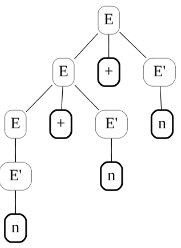
\includegraphics[scale=1]{images/AlberiParsing/associativitaSinistra.png}
      \caption{Associatività Sinistra}
  \end{subfigure}
  \hfill
  \begin{subfigure}{0.45\textwidth}
      \centering
      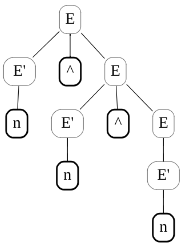
\includegraphics[scale=1]{images/AlberiParsing/associativitiaDestra.png}
      \caption{Associatività Destra}
  \end{subfigure}
  \caption{Confronto tra associatività sinistra e destra}
\end{figure}
 
Quando ho la menata della precedenza, operatori binari con precedenza diversa, questo si trdauce con l'introduzione di simboli ulteriori abbamo or n. Questi simboli sono terminali che rappresentano la precedenza degli operatori.

\begin{lstlisting}
  G_p = Grammar.from_string("""
  E -> E + P | P
  P -> P * F | F
  F -> n
  """)
\end{lstlisting}

\begin{figure}[ht!]
  \centering
  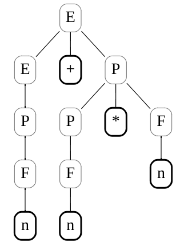
\includegraphics[scale=1]{images/AlberiParsing/precedenza.png}
\end{figure}

Nel caso del dangling else (if else if) diventa una cosa ancora più dolorosa c'è un interplate tra SMUC che è difficile da ricordare risolve la cosa perchè tiene l'else legato all'if più vicino.

\begin{lstlisting}
  G_if = Grammar.from_string("""
  S -> M | U
  M -> if C then M else M | stm
  U -> if C then M else U | if C then S
  C -> cond
  """)
\end{lstlisting}

\begin{figure}[ht!]
  \centering
  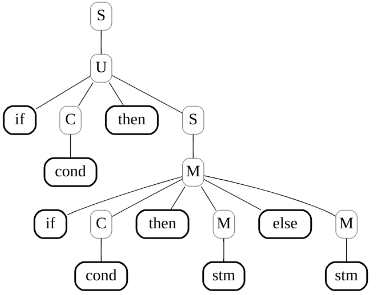
\includegraphics[scale=1]{images/AlberiParsing/dandlingElse.png}
\end{figure}

Il punto cruciale è che context free siamo al giusto livello (non ci siamo persi le parentesi sotto) abbiamo alberi di parsing lineari nella lunghezza della parola, ma dobbiamo stare attenti che avremo ambiguità ed in questo caso dobbiamo o modificare la grammatica che però sarà piena di non terminali e spesso questa procedura passa da trucchi e non c'è niente di teorico (che si possono copiare o inventare).


\chapter{Parsing}
Quello che vogliamo fare ora è passare partendo da un simbolo distinto espandendo una serie di regole per cui alla fine del processo avrò la parola.
L'altro processo è l'opposto parto dalla parola e cerco di capire quali sono gli ultimi pezzi che hanno composto la parola e poi proceso all'indietro fino ad arrivare al simbolo distinto, in questo modo cerco di riaggregare i pezzi andando dal basso verso l'alto.
Questi a grandi linee sono le due strategie che applicheremo per il parsing. I due modi si chiamano:
\begin{enumerate}
    \item \textbf{Top-down}: Parto dal simbolo distinto e cerco di arrivare alla parola
    \item \textbf{Bottom-up}: Parto dalla parola e cerco di arrivare al simbolo distinto
\end{enumerate}

Notiamo che questi approcci possono essere appliacati a tutte le grammatice, ad esempio vediamo una grammatica context sensitive:
\begin{lstlisting}
\end{lstlisting}

Quello che a volte conviene fare è ribaltare la grammatica, le produzioni left producono le right, questo ovviamente va a rovinare la nostra grammatica, poi possiamo mettere anche un simbolo Inizio e Fine per indicare l'inizio e la fine della produzione. Spesso lavorando in questo modo si produce una derivazione right-most (sostituisco il simbolo più a destra della derivazione non sentenziale e sostanzialmente faccio i passi da destra a sinistra dall'ultimo al primo). Posso decidere dall'alto in basso e queso produce derivazioni left-most oppure posso andare dal basso verso l'alto cercando di aggregare e ottengo derivazioni right-most ma che devo leggere dal basso verso l'alto.

\section{NPDA}
In realtà questo tipo di comportamento viene modellato nell'ambito del parsing attraverso la nozione di automa che ha bisogno di un nastro di input ed un area di memoria per tenere il processo di parsing, sostanzialmente deve fare la scansinoe della parola e mano a mano costruire l'albero di derivazione. Tutti gli algoritmi che vedremo hanno bisogno di una pila (stack) come forma di memoria per tenere traccia del processo di parsing perchè il tipo di lavoro che fanno non richiede un accesso causale alla memoria. Ma come fanno a decidere questi automi? hanno un dispositivo di controllo che è in grado di determinare cosa fare, come spostarsi sul nastro e cosa scrivere e prendere dalla pila. La cosa più intuitiva che uno può fare è avere una mente omiscente che è in grado di determinare cosa l'automa in ogni situazione deve fare. Quello che dovremo fare nel nostro lavoro è costruire questo controllo e poi trovare un modo per elminare il non determinismo perchè non avremo l'oracolo che sa tutto.

Quello che accadrà è che data una descrizione della grammatica sarà possibile realizzare la struttura di controllo dell'automa in maniera automatica, potremmo pensare ad un programma che dato in pasta la grammatica G produca l'automa, questi programmi si chiamano \underline{parser generator}.
Un'altro modo molto usuale, che descrive una grande famiglia di algoritmi di parsing, è quello di avere un controllo universale (che funziona per ogni grammatica) trasformando una tabella che rappresenta le informazioni che G contiene in una forma che fa in modo che il controllo sappia cosa fare, questo metodo si chiama \underline{table driven}.

Nell'analizzare il comportamento di questi parser ci sono due grandezze che vogliamo vedere:
\begin{enumerate}
    \item Lo spazio in memoria, quanto spazio consuma l'automa nel funzionamento sempre in rapporto alla lunghezza della parola
    \item Il tempo di esecuzione, quanto tempo impiega l'automa a processare la parola
\end{enumerate}

Evidente più è alto il tipo di grammatica più è alta la memoria e più scendiamo il contrario.
Noi ci occuperemo delle context-free e per quel che concerne gli altri due livelli della gerarchia osserviamo questo:
\begin{itemize}
    \item Le tipo 0 (unrestricted) rappresentano gli insiemi ricorsivamente enumerabili, quindi chiedersi se una parola appartiene ad una grammatica di tipo 0 equeivale a chiedersi se il programma termina, problema indecidibile
    \item Le tipo 1 (context sensitive) sono più deboli delle unrestricted, sono gli insiemi accettati da una macchina di Turing non deterministica, problema decidibile ma non in tempo polinomiale bensì in tempo e spazio esponenziale. Questo è il livello in cui si colloca il parsing naturale (linguaggi naturali).
    \item Le tipo 2 (context free) sono gli insiemi accettati da un NPDA, problema decidibile in tempo polinomiale.
\end{itemize}

Una cosa che vale la pena considerare nell'ambito del parsing context-free esiste una possibile divisione del lavoro che dobbiamo fare raggruppando sulla base di qualche criterio. Una prima grande dicotomia è se gli algoritmi funzionano in maniera:
\begin{enumerate}
    \item top-down
    \item bottom-up
\end{enumerate}

Un'altra dicotomia piuttosto interessante è il modo in cui l'input viene analizzato, perchè l'automa può andare avanti ed indietro nell'input:
\begin{enumerate}
    \item Parser direzionale: L'automa va avanti e indietro nell'input, in ordine, se lo ciuccia man mano che riceve i byte
    \item Parse non direzionale: il parse può adoperare delle porzioni del nastro diverse, ad esempio nell'uso degli editor abbiamo la colorizzazione della sintassi, in questo caso il parser non è direzionale perchè se fosse direzionale dovrei ricostruire tutto l'albero per ogni modifica.
\end{enumerate}

Un'altra possibile dicotomia che abbiamo già in qualche modo accennato è il fatto che purtroppo abbiamo il non determinismo e per risolvere questo potrebbe provare tutti i passi agendo:
\begin{enumerate}
    \item Depth first
    \item Breadth first
\end{enumerate}

Una possibilità cruciali per eleminare il problema del non determinismo è avere un parsing che a priori non accetti qualsiasi grammatica ma solo quelle che sono in una certa forma, quelle deterministiche (si rispippola la grammatica in modo che sia deterministica). Questo ci crea dei parsing molto meno potenti.

Cosa vedermo noi:
\begin{enumerate}
    \item Non directional methods Bottom-up: CYK parser
    \item Deterministic directional:
    \begin{enumerate}
        \item Top-down: LL parser, mescolare parsing e traduzione è più semplice dell LR. Sono meno efficienti ma pace, noi useremo un parser generator LL(*). Noi vedremo LL(1).
        \item Bottom-up: LR parser, vedremo LR(0)
    \end{enumerate}
\end{enumerate}

\section{CYK parser}
L'algoritmo CYK si basa su una tabella che rappresenta la comprensione temporanea che ha l'algoritmo del processo di parsing (della costruzione dell'albero di parsgin) e questa tabella più essere facilmente riempita nel caso in cui la grammatica abbia una forma semplificata che per il momento noi assumeremo. Le regole che vorremo avranno solo questa forma, una produzione non terminale o di una coppia:
\begin{lstlisting}
    A -> BC
    A -> a
\end{lstlisting}

La tabella di questo algoritmo è fatta così, sulla base abbiamo la parola e poi ha una serie di celle in cui in ciascuna cella contiene l'informazione della sotto-parola la cui lunghezza è data dalla riga in cui mi trovo e che raccontano l'idea che si è fatto l'algoritmo di parsing della stringa lunga due a partire dalla posizione della tabella sotto. Nella posizione i,l rappresenta l'informazione che ho sul parsing del prefisso della parola che comincia lì ed è lunga l:
\begin{lstlisting}

\end{lstlisting}

Osserviamo che la tabelle può essere riempita in due modi, siccome ogni posizione riguarda un sottoinsieme la posso riempire in due modi:
\begin{enumerate}
    \item offline: parto dal fondo a sinistra e comincio a mettere le lettere singole, poi sopra le coppie e così visita. Offline perchè per riempirla devo aver visto tutto l'input
    \item online: la riempio in diagonale partendo dal basso a sinistra, mano mano che vedo caratteri posso riempire sempre più celle
\end{enumerate}

\begin{lstlisting}
    
\end{lstlisting}
Noi ovviamente non la riempiremo di parti di parola ma di produzioni, per filtrare le produzioni useremo la funzione di python filter che filtra cose in base ad una funzione che gli passiamo.
Quando siamo in alto nella tabella dobbiamo mettere una produzione che da A produce BC, perchè vogliamo metterci qualcosa che produce quello che c'è sotto quindi sotto dobbiamo andare a vedere se B produce un pezzo di quello che c'è sotto e la C il resto.

In buona sostanza se sono a lunghezza 1 ci metto tutti i terminali dove A produce a dove a è proprio la parola (lettera negli esempi) che sto cercando, se sono a lunghezza 2 metto tutte le produzioni che producono due terminali B e C dove B produce la parola da i a k e c da k in poi.
\begin{lstlisting}
    
\end{lstlisting}

Negli esempi si vede bene che sotto mettiamo tutti i terminali delle produzioni a sinistra che producono la parola o lettera (ad esempio A produce a quindi ci metto A per tutte le volte che ci sono a nella parola). Poi per le celle sopra ci chiediamo se c'è una produzione che produce $A \rightarrow BC$ dove B produce la sotto parola da i a k e C da k in poi (ad esempio $S \rightarrow A, S$).

Per guardare se la parola fa parte del linguaggio basta guardare la cella in alto della tabella, se è riempita significa che è ok.
\subsection{Albero di parsing}
Dobbiamo ricostruire l'albero di parsing da questa tabella, al momento ci accontentiamo di costurire l'albero i cui nodi sono i non terminali e gli archi le produzioni (non ha dentro le produzioni). Non è super difficile perchè possiamo approcciare questa cosa ricorsviamente

\begin{lstlisting}
    
\end{lstlisting}

\section{Elminazione epsilon-regole}
Per eleminare una epsilon regola poteri duplicare la regola, cioè se ho una regola A $ -> \epsilon$ e una produzione B $-> \alpha$ A B posso da qui crearne due con $A_1$ e $A_2$. Non sempre è così comodo. La prima osservazione che facciamo è che abbiamo trasformato G in g primo in cui non abbiamo le epsilon regole ma il costa è che per ogni epsilon regola che eliminiamo produce $2^n$ produzioni (dove n è la lunghezza della regola). Quindi sappiamo che $|G^{'}| \ge 2|G|$.

La prima cosa che dobbiamo fare è il rimpiazzamento di A con $A_1$ in tutte le produzioni, poi prendo tutte le produzioni che contengono A e cancello o sostituisco con A primo le occorrenze di A, se invece on l'ho beccato in B lascio così com'è:
\begin{lstlisting}

\end{lstlisting}

A questo punto per sistemarle dobbiamo fare una chiusura, perchè abbiamo prodotto delle epsilon regole, prende tutti i non terminali che non abbimo ancora visto e se quel terminale tra i lati destri di A c'è una epsilon regola faccio il rimpiazzamento e segno che l'ho fatto.
\begin{lstlisting}
  
\end{lstlisting}

Osserviamo che questo procedimento non ha tolto le epsilon regole ma le ha messe inline, le mette dove accadevano, quello che succede è che queste regole prima o poi diventano unreachable quindi prima o poi questa regola la toglieremo. L'altro effetto è che solleva la epsilon fino al simbolo distinto, quindi quello che accade è che questo linguaggio potrebbe produrre la parola vuota.
Usando i passi precedenti è semplice arrivare al passo di eliminazione:
\begin{lstlisting}
  
\end{lstlisting}

\section{Eliminazione delle unit rules}
Le regole unitarie sono quelle della forma A -> B, cioè una variabile che deriva un'altra variabile. Queste regole sono molto pericolose perchè possono creare loop, quindi la prima cosa che facciamo è eliminare i loop. Quello che mi aspetto in questo caso mi aspetto anche che ci sia una C che deriva B e A che deriva qualcos'altro che non è B. Quello che si fa è in tutte le regole dove c'è la A ci metto tutte le alternative. Dato B -> $\omega_1 | \omega_2$ e $C -> \alpha A B$ posso fare $C -> \alpha \omega_1 | \alpha \omega_2$. Faccio questa sostituzione a meno che non mi trovi nel caso del loop $B -> B$.
Prendo tutte le produzioni che sono lunghe 1, le spacco, dico che A produce B, se B è un non terminale prendo le produzioni e faccio l'inline, faccio in modo che A produca tutte le produzioni di B e poi elimino A produce B:
\begin{lstlisting}
  
\end{lstlisting}

Notiamo che questo porta ad avere una grammatica con delle cose irraggiungibili. Se voglio fare pulizia uso la tecnica dell'altra volta che ancora non è quello da cui siamo partiti perchè ad esempio ci sono dei non terminali oppure delle cose lunghe 3.
Ci rimangono due passaggi:
\begin{enumerate}
    \item Eliminare i non solitari: $A -> \alpha a \beta$. dove alpha e beta non sono termina
    \item Eliminare le produzioni più lunghe di 2
\end{enumerate}

Per ogni solitario che trovo in giro produco una regola unitaria lunga 1 e sostituisco secco, non ho bisogno neanche di fare le chiusure, cerco le produzioni A B e cerco nel lato destro e guardo cosa sono, se sono dei non terminali li lascio come sono, se sono dei terminali li sostituisco con N e la letterina, dopo di che sostitusico la produzione $Na -> a$ ad esempio:
\begin{lstlisting}
\end{lstlisting}

Per le produzioni lunghe faccio produrre ad un prio pezzo x1, x2 poi ad un secondo pezzo A2 faccio produrre A1 x2, così via fino in findo dove avrò A produce A3 x7, partendo da una produzione $A -> x1 x2 x3 x4 x5 x6 x7$:
\begin{lstlisting}
   def make_binary 
\end{lstlisting}

Ora dobbiamo ricostruire l'albero di parsing, ci verrà più facile rispetto a fare una trasformazione di alberi sostituendo la tabella CYK qualcos'altro.

\subsection{Costruzione albero parsing left-most}
Dato un certo non terminale ci diamo come obiettivo costruire un fattore di una parola di input che partiva da una certa posizione con una certa lunghezza.
Se la lunghezza è 1 devo andare a cercare una produzione della forma X i -1, questa cosa funziona perchè la tabella è costruita correttamente. Se andiamo a riprenderlo è uguale a fake parse, non metto gli alberi ma metto le produzioni:
\begin{lstlisting}
    
\end{lstlisting}

Bisogna considerare anche cosa succede nelle produzioni non binarie, mi piacerebbe avere una funzione derives che prende una sequenza di simboli, una i e una l e restituisce una serie di lunghezze ln tale per cui l0 è la lunghezza derivata da w0 input i + i + l0. Per farlo dovrà fare una ricorsione sulla tabella.
Mi sono perso mannaggia a me, ma era abbastanza inseguibile, prova a vedere dal libro.

\chapter{ANTLR}
ANTLR e' un parser generator che genera un parser LL top down multi linguaggio. A partire da una grammatica possiamo generare il parser nel linguaggio che vogliamo e ci genera un runtime nel linguaggio che vogliamo per fare funzionare il parser.

La roba interessante e' che ci sono un sacco di grammatiche pronte per ANTLR.

Abbiamo due modi per usare questo strumento:
\begin{itemize}
    \item Uso diretto di ANTLR, leggendo il manuale e capire come funziona per scrivere il codice python
    \item Uso mediato da Liblet, significa che il prof ha scritto un po' di codice in Liblet che serve per importare roba di Java in maniera dinamica
\end{itemize}

Nel progetto e' una delle cose che possiamo scegliere.

\section{Uso diretto di ANTLR}

La cosa principale di questo strumento e' che ci permette di specificare la grammatica context free che vogliamo usare per produrre il parser tramite file o stringa. Questa grammatica e' fatta cosi', definiamo la grammatica, poi ci sono una serie di regole di tokenizzazzione scritte in maiuscolo alla cui destra c'e' una espressione regolare. Le regole della grammatica (di parsing) iniziano in minuscolo, sono date da un simbolo di tokenizzazzione e poi si possono mettere delle costanti.
Alcuni token possono essere scartati dalla parte di parsing.

\begin{lstlisting}
    
\end{lstlisting}

Adesso il punto cruciale e' utilizzare un tool Java che generi codice Python. Lui genera 4 file:
\begin{itemize}
    \item lexer
    \item parser
    \item visitor: interfaccia che permette di visitare il tree generato dal parser
    \item listener: interfaccia
\end{itemize}

%Esempio di uso

Uso del lexer, possiamo vedere i passi del lexer, il token ci fa vedere anche i caratteri del sorgente che rappresentano il token:


Abbiamo visto un esempio piu' complesso di una grammatica di espressioni ed assegnamenti. Vediamo ora come usare il paser, tendenzialmente i parser hanno due modalita' di funzionamento:
dato che l'albero e' una struttura ricorsiva ci sono due modi per poterne fruire. Ognuno di questi nodi e' relativo ad una delle regole di parsing, i figli sono i token.
\begin{itemize}
    \item listener: ha due metodi per ogni regola, entro ed esco. Poi posso invocare un processo di visita che invoca il listener secondo l'ordine che mi aspetto.
    \item visitor: me lo scrivo io, mi scrivo una funzione per ciascuna regola che sono quelle usate per fare la visita.
\end{itemize}

Quello che faremo noi a lezione e' usare visitor, perche' a lezione usando LIBLET ci dara' un albero e noi ci scriveremo sempre le visite dell'albero.
Cosi' e' come useremo il listener, creo una classe che implementa il listener, poi creo l'istanza e lo passo al walker di liblet che lo usa per fare la visita:
\begin{lstlisting}

\end{lstlisting}

Nel caso del visitor ho sempre la mia classe che implementa il vistor, mi implemento dentro la visita e poi uso la classe per fare la visita che mi sono scritto:
\begin{lstlisting}

\end{lstlisting}

Fino ad ora non ci siamo mai occupati degli errori, ma in caso di ANTLR si possono specificare degli ascoltatori di errore che hanno un metodo che va invocato ogni volta che lui vede un errore nel lexing o nel parser:
\begin{lstlisting}

\end{lstlisting}

\section{Uso mediato da Liblet}
Il modulo ANTLR dentro Liblet ci permette di prendere una grammatica e mi da un oggetto che ha delle competenze.
In questa grammatica ci sono delle etichette di ANTLR che ci servono a distinguere le alternative di una regola che ha delle alternative che e' comodo perche' se avviene un match di stat non sapremmo cosa abbiamo matchato:
\begin{lstlisting}

\end{lstlisting}

Dato l'oggetto possiamo fargli fare diverse cose, inizialmente vediamo i tokens, basta un metodo in questo caso:
\begin{lstlisting}

\end{lstlisting}

Posso avere anche il contesto, che mi da dove partire per il visitor, posso dargli anche il token da cui partire:
\begin{lstlisting}


\end{lstlisting}

L'albero di parsing possiamo produrlo con un metodo tree che produce un tree di liblet con dentro le espressioni:
\begin{lstlisting}

\end{lstlisting}

ANTLR accetta anche grammatiche malate (ricorsivita', precedenze...) c'e' pero' una malattia che non puo' essere riconosciuta a tempo di analisi, la ambiguita'. Si puo' accendere una spia che ci dice se il parsing e' ambiguo, il suggerimento e' che quando si progetta una nuova grammatica si preparano dei testcase e vedo se il diagnostici mi dice se e' la grammatica e' ambigua. Va acceso il diag = True nel context:
\begin{lstlisting}

\end{lstlisting}

%manca tutta la prima parte della lezione 16, sono arrivato tardi

\subsection{Grammatiche note}
Possiamo guardare alcune grammatiche note che possono essere utili, ad esempio c'e' una grammatica per l'aritmetica, bella ma l'associativita' a destra la sbaglia.
Un'altra grammatica carina e CALCULATOR, che parsa le espressioni e permette l'invocazione di funzioni, come il seno o coseno.

Un'altra grammatica super utile, che non viene dal repository standard, ma dal libro di antlr e' la grammatica del linguaggio Cymbol che e' una specie di linguaggetto di programmazione che ha l'invocazione a funzione e gli statement.

La fine di questa cosa e' che e' molto potente, e se incontriamo errori guardiamo in documentazione perche' ci sono alcune porcherie.

\subsection{Ancora su listener e visitor}
Ora ci assegniamo due compiti ed useremo listener e visitor per fare due cose diverse:
\begin{itemize}
    \item Numerare le righe
    \item Interpretare un linguaggio
\end{itemize}

Il linguaggio a cui faremo riferimento e' il linguaggio aritmetico con nomi di variabili ed assegnamenti. Una sequenza lineare di istruzioni in cui le istruzioni sono assegnamenti, stampe o espressioni.

%grammatica e programma

Vogliamo contare gli assegnamenti, lo faremo con un listener, sappiamo che ANTLR ci da' un listener che e' un interfaccia da estendere, noi lo estendiamo e implementiamo i metodi che ci interessano. In questo caso ci interessa il numero di assegnamenti, quindi implementiamo il metodo che ci interessa. Poi creiamo un oggetto del listener e lo passiamo al walker di liblet.

\begin{lstlisting}

\end{lstlisting}

Ora vogliamo interpretare il programma, un compito cosi' sofisiticato spesso si realizza piu' facilmente con un visitor, perche' quando scrivo un linguaggio ho in testa per ogni nodo del linguaggio cosa voglio fare, in particolare noi vogliamo che per ogni nodo restituisca il valore del nodo, questo lo puo' fare facilmente se fa una visita in post-ordine conoscendo i valori dei figli.

In questo caso abbiamo solo variabili locali, quindi la cosa piu' facile da fare e' tenere una memoria che e' un dizionario di python, se vediamo un assegnamento prendiamo il nome della variabile, facciamo lo scarico ricorsivo chiamando expr e salviamo tutto in memoria. Se vediamo una variabile, facciamo un lookup in memoria e restituiamo il valore. Se vediamo un numero lo restituiamo direttamente, da notare che quando restituiamo l'intero e' l'unico passo interpretativo perche' stiamo trasformando testo in intero. Abbiamo un espressione che fa la print, non ritorna niente ma fa una print. Dopo di che c'e' la parte di associazione, di nuovo sono divise perche' sono cose divise, in ogni caso visito tramite scarico ricorsivo il lato sinistro e destro e poi guardo il tipo dell'operatore, la visita delle parentesi e' un trucco sintattico che serve ad indicare diverse precedenze, quindi dal punto di vista interpretativo non serve a niente e si puo' solo mangiare.
%perche' due metodi per la somma e la moltiplicazione? 
\begin{lstlisting}

\end{lstlisting}

Estendere questo parser su linguaggi piu' difficili e' immediato, la logica e' sempre la stessa, basta estendere le regole di parsing e le regole di interpretazione. Potrebbe essere un buon esempio. Il trucco cruciale e' che il visitatore e' ricorsivo quindi posso quando ho un dubbio su che cosa fare posso usare la ricorsione, per valutare un espressione valuto ricorsivamente i figli e poi faccio l'operazione.
Il problema di questa cosa e' che la pila di chiamate ricorsive puo' esplodere e non e' facile da tenere sotto controllo, soprattutto se vogliamo dare degli errori durante il parsing. Quindi abbiamo bisogno di fare una traduzione in cui rendo la ricorsione esplicita, significa liberarsi della ricorsione passando ad una struttura iterativa, significa avere una pila di chiamate esplicita invece della pila di record di attivazione, l'idea qui e' che tengo dei risultati parziali. Qui dobbiamo scegliere tra visitor che usa la ricorsione e listener in cui teniamo una pila esplicita per le chiamate.

L'idea in questo caso e' di tenere gli operandi sulla pila e quando siamo pronti a fare l'operazione togliamo gli operandi e mettiamo il risultato intermedio.
Quindi il listener avra' due strutture dati per funzionare, una memoria per le variabili ed una pila. Qui ho bisogno degli exit perche' voglio sapere cosa fare con quello che c'e' sulla pila dopo che ho guardato i figli. Se usciamo da un assegnamento significa che ho gia' valutato l'espressione e sulla pila c'e' il valore da assegnare, quindi assegniamo in memoria. Se usciamo da un id o un intero significa che valutiamo il valore e mettiamo sulla pila il valore. Quando usicamo da una divisione mi aspetto che i valori dei suoi operandi siano sulla pila messi dalla visita in post-ordine, quindi li tolgo dalla pila e metto il risultato della divisione sulla pila. Se usciamo da una somma invece mettiamo il risultato della somma sulla pila.

\begin{lstlisting}

\end{lstlisting}

\section{Dall'albero di parsing all'AST}
L'idea e' di partire da un albero di parsing che ha tanti artefatti, toglierli e raggiungere una forma compatta che e' un abstract syntax tree. Per farlo usiamo una funzione ricorsiva.

Abbiamo visto che in ANTLR si puo' mettere del codice direttamente nella grammatica, non lo faremo mai e' troppo doloroso, poi non ha troppo senso tenere legata la grammatica con l'implementazione del parser.

\subsection{Dispatch table}
Useremo una dispatch table per capire cosa fare quando troviamo una regola (nella table ci saranno le funzioni ricorsive). Inizialmente diciamoche quando troviamo una regola e c'e' nella dispatch table chiamo la sua regola, se non la trovo metto tutti in un catchall:
\begin{lstlisting}
    
\end{lstlisting}

Devo riempire la tabella, in questo caso definiamo le funzioni che ci servono quando vediamo gli operatori, da notare che come scarico ricorsivo non usano se stesse ma chiamano la funzione che usa la dispatch table, poi popolo la table:
\begin{lstlisting}
    
\end{lstlisting}

Si e' visto che liblet implementa una classe TreeWalker che fa questo lavoro della funzione ricorsiva, possiamo dirgli dato un albero che attributo considerare, registrare delle funzioni che usa quando incontra dei simboli (con un annotazione o registrarle esplicitamente), inoltre permette anche di avere un catchall (ne esistono di tanti tipi).

Vediamo un esempio in cui eseguiamo il programma partendo da un ATS, notiamo che occupandoci degli atomi abbiamo solo const e var, non abbiamo bisogno di castare ad Int perche' lo abbiamo gia' fatto nella costruzione dell ATS quando mettevamo dentro il valore di una costante.

\begin{lstlisting}
    
\end{lstlisting}

\section{Trasformare}
Vediamo alcuni esperimenti di trasformazione, in particolare inizialmente vogliamo trasformare un documento JSON in un documento HTML usando ANTLR.

Quello che facciamo noi e' modularizzare il processo, partiamo generando l'AST, si fa con un tree walker ricorsivo che ha la tabella di dispatch che discrimina i nodi in base al nome.

\subsection{Trasformare HTML in matrici}
L'idea e' che ho acceduto ad una pagina HTML con dentro delle tabelle e io voglio farmi una matrice che rappresenta i dati, e' una trasformazione di dominio.

Per farlo partiamo con il definirci una nostra grammatica invece di usare quella completa assumendo per semplicita' che dentro i td possano esserci solo interi.

Il processo e' sempre lo stesso, arriviamo all'AST e qui la cosa che cambia e' che per fare la trasformazione usiamo una struttura dati esterna, uno stack, quando vediamo i dati li pushiamo dentro lo stack e quando vediamo una row togliamo i figli e li mettiamo dentro un array, alla fine dello stack avremo un array di array che rappresenta la matrice.

Abbiamo visto anche che per costruire la tabella potremmo pensare di decorare i nodi con il numero di riga e colonna mettendo nella radice il numero di righe e colonne, cosi' posso poi precomputare una matrice di dimensioni fisse piena di None e poi riempirla visitando l'AST.

\section{Traspilazione}
L'idea e' quella di prendere un linguaggio e trasformarlo in un altro linguaggio. Questa cosa ha origini storiche perche' ad esempio il C non veniva compilato ma traspilato in Fortran. Ci sono anche logiche di portabilita' e di ottimizzazione. La portabilita' e' moderna, uno dei linguaggi dominanti nel web e' JavaScript, il problema di questo linguaggio e' che non e' standardizzato e non coinvolge tutti i browser. Ragione per cui e' nata una famiglia di traspilatori che prendono un JS recente e lo trasformandono in un JS piu' vecchio che gira su tutti i browser. Un esempio e' Babel, che e' un traspilatore di JS, ma ce ne sono anche altri. Se esistono costrutti che nelle vecchie versioni non esistono si usano gli SHIM. E' nato anche typescript, che non esiste nei browser, ma viene traspilato in JS.

Noi partiamo da un linguaggio semplice SimpleLang, prima lo traspiliamo in JavaScript (facendo un text to text trsaplilazione). L'altro passo che faremo e' quello di sfruttare il fatto che alcuni linguaggi hanno una rappresentazione di alto livello, ma che e' un po' piu' snella di un testo (non richiede ulteriori processi di parsing) che puo' essere complata dalla VM e generata senza troppo sforzo, quindi tradurremo questo linguaggio verso Python facendo una traduzione da testo verso l'AST di python (AST = Abstract Syntax Tree).

Dobbiamo decidere come fare l'IO, perche' ha senso compilare un programma solo se c'e' un input. Noi per farla facile cercemo di provvedere modi banali per dare l'input ai nostri programmi, l'interprete preleva delle cose dal mondo esterno e le inietta nel programma. Nel nostro caso assumiamo che ci siano tre variabili INPUT e per farla facile faremo che ha un solo OUTPUT. (dice che il progetto di quest'anno non avra' bisogno di librerie esterne).


Arrivati infondo alla traspilazione dobbiamo cercare di valorizzare la variabile INPUT, facciamo una funzione che cerca tutti gli input e per ciascuni di essi apre un prompt che prende l'input.

Vediamo ora come cercare di evitare il passo di parsing del linguaggio in cui arriviamo. Scriviamo il linguaggio in una forma in cui l'interprete di python sia in grado di interpretarlo direttamente, python perche' e' fornisce delle API per interagire con gli AST.
Si puo' usare eval per fare valutare una funzione e generare un parse tree. una volta che abbiamo un AST possiamo compilarlo con la funzione complie di python che vuole sapere cosa sta compilando e in che modalita'.
Per fare la traspilazione verso l'ATS di python dobbiamo visitare il nostro albero e trasformare i nostri nodi nei loro corrispondenti nodi di python.

Dopo siamo di nuovo nella situazione di dover valorizzare gli input, i programmi di python hanno un dizionario dove pesca le variabili locali, noi possiamo aggiungere con un dizionario di python le variabili che ci servono. Ora li stiamo mettendo a mano noi, potremmo anche pensare di mettere delle funzioni per valorizzare le variabili di input.

\chapter{Progetto}
L'idea e' quella di ragionare sulla ricorsione investigando la questione che la ricorsione e' una cosa potente ma costosa. Saltino e' un linguaggio che non ha iterazione, se non ho iterazione devo fare la ricorsione.
Il punto e' che esistono una serie di strategie per mitigare questo approccio, un esempio di somma senza ricorsione:

\begin{lstlisting}
    Somma(n){
        if n == 0 {
            return 0
        } else {
            return n + Somma(n-1)
        }
    }
\end{lstlisting}

Quando la ricorsione e' l'ultimo passo e' facile trasformare la ricorsione in iterazione. Questa cosa si chiama tail recursion, elimini la ricorsione con un while true in cui riassegno quello che ho sulla pila dello stack nel caso della ricorsione, deve essere l'interprete a fare questa cosa.

Quindi l'idea e' inizialmente implementare un interprete ricorsivo e poi implementare un linguaggio saltone che non ha ricorsione, eliminando la ricorsione con un while true eliminando la ricorsione di coda.
Ocio che con la somma non funziona quella cosa che dicevamo, la ricorsione non e' l'ultima cosa che faccio, devo ritornare i risultati parziali, ma devo ritornare degli accumulati, di fatto mi porto la somma parziale come secondo argomento:
\begin{lstlisting}
    Somma(n, acc){
        if n == 0 {
            return acc
        } else {
            return Somma(n-1, n+acc)
        }
    }
\end{lstlisting}

A questo punto posso scrivere con un while true:
\begin{lstlisting}
    Somma(n){
        acc = 0
        while true {
            if n == 0 {
                return acc
            } else {
                new_n = n -1
                new_acc = n + acc
                n = new_n
                acc = new_acc
            }
        }
    }
\end{lstlisting}

Ha detto che fare l'interprete iterativo rende molto facile la trasformazione in saltone, ovvero togliere la ricorsione.

Gli errori devono essere trappati, non devono vedersi stack trace di python.
\end{document}